\documentclass{myBeamer}

%% Title page
\title{Ordinary Differential Equations}
\subtitle{as an alternative to agent-based modelling}
\author{Module}
\date{\today}
%\institute{Institut\\
%\bigskip
%
\includegraphics[scale=2]{figures/logos/openmole.png}}


\begin{document}

\begin{frame}[plain]
	\titlepage
\end{frame}
\addtocounter{framenumber}{-1}

\AtBeginSection[]
{
	\frame{
		\sectionpage
	}
	\addtocounter{framenumber}{-1}
}


\section{ODE systems}

\sframe{The ODE framework}{
	$\rightarrow$ widely used to model transmission phenomena\\
	
	\bigskip
	
	\begin{columns}
	\begin{column}{.5\textwidth}
		\begin{itemize}
			\item population split into compartments
			\item system of ordinary differential equations
		\end{itemize}
	\end{column}
	
	\begin{column}{.5\textwidth}
		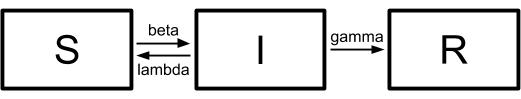
\includegraphics[width=\textwidth]{figures/SIR.jpg}\\
		
		\begin{eqnarray*}
		\left\{
		\begin{array}{lcl}
			\dv{S}{t}  & = &  -\beta S + \lambda I \\
			\tmspace{1mu}&& \\
			\dv{I}{t} & = & \beta S - (\lambda + \gamma)I \\
			\tmspace{1mu}&& \\
			\dv{R}{t} & = & \gamma I
		\end{array}
		\right.
		\end{eqnarray*}
	\end{column}
	\end{columns}
}


\sframe{SIR model dynamics}{
	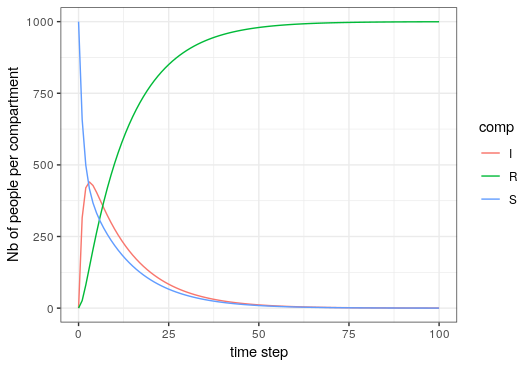
\includegraphics[width=\textwidth]{figures/SIR_dynamics.png}
}


\sframe{ODE vs ABM}{
	\begin{table}
 	\begin{tabular}{ll}
 		\thead{\head{ODE}} & \thead{\head{ABM}} \\
		Equation-based & Individual-based \\
		Generic mechanisms & Precise mechanisms \\
		Population scale & Individual scale \\
		Needs less resources & Computationally  expensive
  	\end{tabular}
  	\end{table}
}


\section{A Zombie situation}

\sframe{An ODE model for our Zombie problem}{
	\head{How could we model the Zombie invasion?}
	
	\begin{itemize}
		\item Which mechanisms?
		\item Which parameters?
	\end{itemize}
	
	\bigskip
	
	\visible<2>{
	\head{How can we assess our model's ability to reproduce the real data?}
	
	\begin{itemize}
		\item Which metrics?
		\item Which fitness function?
	\end{itemize}
	}
}


\sframe{A very simple ODE model}{
	\begin{center}
	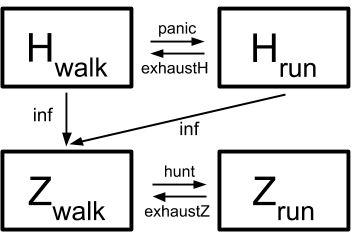
\includegraphics[width=.7\textwidth]{figures/simpleODE.png}
	\end{center}
}


\sframe{A very simple ODE model}{
	\begin{center}
	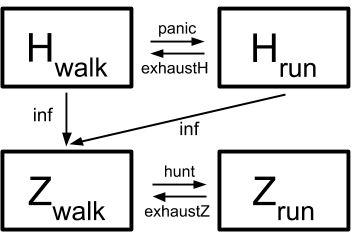
\includegraphics[width=.35\textwidth]{figures/simpleODE.png}
	\end{center}
	
	\begin{eqnarray*}
		\left\{
		\begin{array}{lcl}
			\dv{H_{walk}}{t}  & = &  -(panic + inf) * H_{walk} + exhaustH * H_{run} \\
			\tmspace{1mu}&& \\
			\dv{H_{run}}{t} & = & panic * H_{walk} - (exhaustH + inf) * H_{run} \\
			\tmspace{1mu}&& \\
			\dv{Z_{walk}}{t} & = & inf * (H_{walk} + H_{run}) - hunt * Z_{walk} + exhaustZ * Z_{run} \\
			\tmspace{1mu}&& \\
			\dv{Z_{run}}{t} & = & hunt * Z_{walk} - exhaustZ * Z_{run}
		\end{array}
		\right.
	\end{eqnarray*}
}


\section{Exploration}

\sframe{First step: Calibrate}{
	\begin{center}
	We have some real time series of zombie invasion \\
	$\rightarrow$ find the parameter values to best fit them
	\end{center}
	
	\bigskip
	
	\visible<2->{
	\head{Process}
	
	\begin{itemize}
		\visible<3->{\item Embed the model in OpenMOLE}
		\visible<4->{\item Define a fitness function}
		\visible<5->{\item Write a calibration task}
	\end{itemize}
	}
}


\sframe{Calibration results}{
	\head{Parameter set} \\
	
	\bigskip
	
%	\includegraphics[width=\textwidth]{figures/calib.png}
}


\sframe{Second step: Profiles}{

}


\section{Adding complexity}

\sframe{New mechanisms}{
	\begin{center}
	\head{What mechanisms could we add to better represent the complexity of our Zombie situation?}
	\end{center}
	
	\bigskip
	
	
}


\sframe{Study our model's parcimony}{

}


%% Stop numbering
\backupbegin

\appendix
%\begin{frame}[plain]{Acknowledgements}
%	\begin{center}
%	\head{Lab:}\\
%	
%	\medskip
%	XXX\\
%	\medskip
%	YYY\\
%	\medskip
%	ZZZ\\
%	
%	\bigskip
%	Logos
%	\end{center}
%	
%	\visible<2>{
%	\bigskip
%	\begin{LARGE}
%		\begin{center}
%		\head{Thank you for your attention!}
%		\end{center}
%	\end{LARGE}
%	}
%\end{frame}

%\input{parts/backup}

\backupend

\end{document}